\section{Literature Review}
In this section we will discuss the relevant scientific literature about 
drone control using RL and methods to perform follow-me behavior. 

\subsection{Object Tracking Methods} \label{baselineliterature}
The implementation of RL algorithms in the context of drone control 
is not novel \cite{FrontalViewRL, DroneRLUsingTransferLearning, iowamasterthesis,AirSimDroneNavigation, 
DeepRLforNavUsingSensor, RLfortakeoff, RLenLSTMfordrone}. 
Studies have shown that the use of RL in a variety of situations provide a 
number of benefits. First, with their experience-driven learning process, RL agents 
show a potential to handle complex and dynamic environments \cite{DeepRLforNavUsingSensor}.
In studies where these agents have been allowed to learn inside of a variety of environments, 
they have been able to teach themselves adaptive behavior to solve a required task. 
Such abilities are beneficial, especially in situations where the tasks involve 
the need to track dynamic objects. However, the 
strong point here is that the need to predevelop all the behavior of an agent to 
solve a certain task is being replaced by the development of the learning environment. This 
not only removes the limitations which are posed by preemptively predicting what situation an 
agent might encounter, but also removes possible constraints in behavior that such an agent could 
form. RL agents are notorious for behaving differently than expected \cite{rlisweird}.
Such features can sometimes be a detriment when very specific behavior is required, 
however, they can also be advantageous. In situations where the behavior needs to be adaptive 
and flexible, being able to find new ways in which to reach the goals can be beneficial. 

Another advantage is that machine learning, and by extension RL, is able to generalize 
its learned behavior to new situations \cite{RLenLSTMfordrone}. Generalizability is 
especially crucial when developing agents that should function in a variety of 
environments. In the context of dynamic object tracking, such a feature is critical since 
being able to predict every situation that a drone must handle is complicated. 
Having access to an agent that is able to deduce appropriate behavior in 
a multitude of new situations from the learning process is very relevant. This is 
also something which RL agents have been shown to be able to 
perform to some extent. 

There have been other methods that have been applied in the context of tracking 
objects, or people specifically \cite{DroneFollowUsingPhone, acousticdronefollower, DroneFollowMobileObject, VisualGPS}. 
These methods employ a variety of technologies to improve the object detection, 
object tracking and decision-making process capabilities of a drone. Additionally, 
they have shown 
to be able to fulfill the task successfully. Furthermore, the action-selection 
process is a straightforward goal oriented algorithm that focuses on making sure the 
target object is centered in its view. The additional technologies are introduced as a means to 
target behavior in irregular situations or to improve the overall stability and reliability 
of the information which this algorithm uses. The aforementioned advantages of using RL 
agents are still very applicable to the action-selection process in these suggested 
algorithms. The ability to be 
flexible and adaptive still provides robustness to an agent to new situations and could 
potentially also remove the need for more intricate technologies to be added to a 
drone altogether. For these reasons, research into what role RL could take in 
the development of agents that control drones in dynamic object tracking tasks 
is still relevant. 

\subsection{Reinforcement Learning and Follow-Me Behavior}
Within the field of RL, there are a variety of algorithms to choose from to perform 
the learning process \cite{A3C, DDPG, PPO, SAC, DQNDeepmind, policygradients}. Many of these are 
state-of-the-art algorithms in RL domains and have generally shown 
very promising results. However, the more foundational algorithm of $Q$-learning is still 
a widespread introductory method throughout a variety of exploratory studies \cite{DQNasBenchmark}. 
Overall, $Q$-learning algorithms employ a tabular representation of the action-selection procedure, 
which is characterized by determining an appropriate action for each possible state. Such 
methods are simple to implement and provide ample insights into how an RL agent functions 
inside new domains. Next to this, when conditions are right, DQNs have shown to converge 
definitely to an optimum \cite{DQNprovedConvergence}, therefore lending itself well 
to perform tests with in differing environments. 

Many studies 
have explored methods to which RL could be used in the case of drone control \cite{DroneRLUsingTransferLearning, 
iowamasterthesis,AirSimDroneNavigation, DeepRLforNavUsingSensor}. Nonetheless, 
a problem is that many of these studies have only investigated 
specific tasks to be learned by the RL agent. For example, one such task is the navigation  
through different types of environments \cite{DroneRLUsingTransferLearning, AirSimDroneNavigation, 
DeepRLforNavUsingSensor, ObstacleAvoidance}. Others focus more on very specific movements of 
drone control, such as taking off and landing the device \cite{TakeOffFlyForwardusingRL}. 
Many of these studies have shown the strong positive aspect of using RL in these tasks. 
There is still the questions whether the task of object tracking could benefit from 
RL algorithms, more preferably even: person tracking. There have been some efforts 
to investigate this issue \cite{RLenLSTMfordrone, DroneschasingDrones}, showing promising 
results.
However, RL is very sensitive to environmental variables. The definition of state-spaces, 
action-space and reward function are crucial aspects that determine what behavior will 
be learned and how well these algorithms are suited for such a task. 
Each of these aspects merit some further attention.

\subsection{Reinforcement Learning Elements}
The development of RL agents is synonymous with defining each aspect of the RL domain 
in which the agent will operate. Each of these will be discussed further. 

\subsubsection{Reward Engineering}
First and foremost, the reward signal is the foundation for the learned 
behavior in RL. The reward can be equated with the goal of the agent themselves, such  
that the problem is captured in a formal sense \cite{RLBook}. The definition of a reward function 
therefore becomes crucial in the process of training an agent with a 
behavioral goal in mind. However, defining the reward brings with it 
some challenges that need to be addressed. One such challenge is the trade-off 
between how much predetermined information is implemented in the reward function and 
how much is left open \cite{rewardshaping, sparserewardsarebetter}. The provision of this information 
happens in the sense 
that the reward function specifies some intermediary states as being more desirable 
compared to others, as to achieve a goal. Following this hierarchy, the agent is forced to 
learn the behavior in a specific way, confined to these constraints. 
However, the disadvantages of creating such an ordering is that it 
requires domain-specific knowledge about when an agent is closer to the goal or not. 
This imbuing of some predetermined knowledge in the reward function also blocks 
the agent from finding new ways to solve the problem and is a problem in 
situations where the set of permissible behavior is not known prior to training. 
Next to this, such reward functions are extremely sensitive to small mistakes in 
the order of states, leading to sub-optimal performance \cite{nonsparserewardissuboptimal}. 

The alternative leads to a simplified reward function, where the goal states 
have been marked with a positive signal, and the remainder with a neutral or negative one. 
A problem here, however, is the sparse nature of the reward space. Having a small 
set of states which produce a positive signal in a 
larger state-space means that there are large swaths of states where no signal 
is given. This means that during the exploration of the state-space, it becomes 
harder for the agent to find states where a positive signal is observed. 
Next to this, the previously mentioned problem of unexpected behavior that 
RL algorithms suffer from also becomes more relevant \cite{rlisweird}. With 
predetermined hierarchy in states, the freedom of an agent to develop 
completely new sets of behavior that still optimize the reward function 
is less likely to occur. However, with a sparse reward function, the agent 
is much more likely to develop unexpected behaviors.

Nonetheless, these advantages with using sparse rewards, combined with the latest 
technologies in improving the training processes of RL algorithms in 
such environments \cite{HER}, does lend this method of reward engineering 
to new training avenues.  

\subsubsection{Environment Selection}
The choice of environment in which the agent will be trained, is another 
important aspect for the problem definition. These can vary from either 
neighborhood type environments \cite{AirSimDroneNavigation}, to indoor 
hallways and rooms \cite{DroneRLUsingTransferLearning}, to more 
simplistic abstract environments \cite{iowamasterthesis}. There is a clear 
trade-off between the use of simplified abstract environments compared to 
more complex environments. The degree to which a neural network is able 
to generalize is not endless and placing an agent in a completely different 
environment than which it was trained in, can cause issues in its performance. 
Additionally, using more specific environments also limit the agent's 
generalization capabilities, because of the specificity of the encountered 
situations during training time. Previous attempts at testing 
the generalization abilities of RL algorithms in complex situations. These tests 
have shown that there is a large 
potential for learned behavior to transfer to new environments \cite{DroneRLUsingTransferLearning}.
However, there are a number of issues that are still unresolved. First, 
the environments that have been tested are mostly similar in complexity. Generalizability is 
especially interesting when training can be performed in more simplified environments
and knowledge can be transferred to more complex situations. This problem is also 
dependent on the way the agent perceives the environment through its state 
input. Training agents with normal (RGB) camera inputs, as performed in this study, can bring the added 
problem of having the agent be unfamiliar with similar situations but differing 
color spaces. Therefore, there is still room to investigate whether other 
state-representation could potentially relate the same information without 
encountering these problems. 

\subsubsection{State-space Representation}
The manner in which the state is being represented is a crucial element in agent training 
\cite{staterepresentation}.
As has been showed before, the state representation can be a problem when it comes to 
multiple aspects of the RL agents, including their generalizability 
\cite{DroneRLUsingTransferLearning}.
Good state selection is the basis on which the agent can perceive its environment, but it
also determines what information it can use for its decision-making. An important point is 
to make sure that the relevant information is being fed to the agent. Relevant information 
should include important aspects that influence the reward signal throughout the world. If 
the agent does not receive any input about important conditions that determine the reward 
signal, it is not able to change its behavior in order to optimize this signal. When 
specifically considering the task of follow-me behavior, the object to be tracked is dynamic. 
This means that there are different movements from the target that can lead to obscure the target object. 
This thesis will specifically look at two options with which to improve the agent's ability 
to track such a dynamic object. \newline

\noindent
\textbf{Directionality} \label{directionality} \newline 
The dynamic movements of a person can lead to the person being obscured by obstacles. 
Obstacles such as corners and walls
might be potential pitfalls for the drone with which it should be able to deal with. 
There is a need for the agent to be able to anticipate the movements from the target object, 
in order to reposition itself accordingly to avoid losing the person from its view. In this case, 
a sense of directionality of the 
person is what is required. For this, there are two ways with which to imbue the agent 
with this information. 

The latest state-of-the-art approaches to this issue use Recurrent Neural Networks (RNNs) 
as a means for an agent 
to perceive some sense of change in time series inputs \cite{RLenLSTMfordrone, LSTMinRL}. 
RNNs are neural networks where the outgoing signal of a neuron or layer is used as an input for 
that same neuron or layer during the next pass-through. 
The specific structure of which activations are re-used as inputs vary with different techniques, 
but the overlapping feature is that the neural network receives the activations of previous 
inputs when performing a feed forward the network. This means that the 
network is able to gather patterns from combinations of inputs, instead of only one. 
In the context of RL, this means that the network is now capable of making decisions 
taking into account previous moments as well. In some applications, this has been used 
as a means for the model 
to sense the direction of a target object and decide on an action. 
An unfortunate disadvantage of using RNNs is that they are computationally more complex
and exhaustive than CNNs \cite{comparisonofarchitectures}. This impediment not only reduces 
inference times, which could severely curb overall performance of the agent, but also reduces 
training times. 

There is, however, a simpler more straight-forward approach, 
that can be used. Instead of changing the architecture of the underlying neural network, 
the state could also be represented as a video, or a stack of frames. Feeding such a stack 
of frames can also communicate the movements of the objects 
in a state. This approach can also be done in RL, as the video input of a couple 
of seconds can be used to feed forward through the network and is not an unfamiliar
method. Basic RL problems have been solved applying this method \cite{rlsolvingatari} and 
it is a preliminary alternative to using more 
state-of-the-art approaches \cite{DepthAndStackResearch}. Such state-representations 
require minimal changes to architecture and methodology while still being able to communicate 
the required information to the agent. \newline
 
\noindent
\textbf{Depth Sensing} \newline 
Next to receiving information about the direction of the person, there is also the need to 
perceive the surrounding objects. To achieve follow-me behavior in environments with obstacles, 
the agent should receive some information about its position in relationship to objects in its 
vicinity. 

There are multiple ways in which to communicate distances to drone devices \cite{acousticdronefollower, DepthAndStackResearch}. 
However, keeping to the constraints of using only camera inputs, as described in Section 
\ref{limitations}, the use of computer vision techniques is the most obvious method to solve 
this problem. One such technique is the creation of a depth map, as can be seen in Figure \ref{im:depthexample}.
Depth maps are constructed by representing each pixel by the distance from the camera to the 
object that is in that specific pixel. The resulting image, is one where an agent can 
perceive its distances to all the objects in its FoV. In this example, the darker the pixel, 
the farther away that object is.

\begin{Figure}
    \centering
    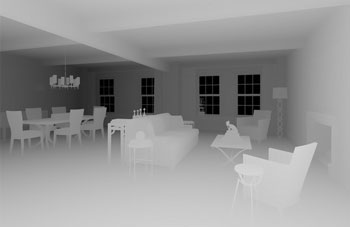
\includegraphics[width=0.6\linewidth]{literature/depth.jpg}
    \captionof{figure}[Example of a depth image]{Example of a depth image \cite{depthimageexample}}
    \label{im:depthexample}
\end{Figure}

Even though there are multiple technologies that can be used in order to calculate these 
distances \cite{lidarinselfdrivingcar, stereovision, DepthFromMonocularImage}, they still have 
the similarity of culminating those distances in the form of a depth map. These can then be 
used in a variety of applications, one of which could be an RL agent. 

Using depth maps as a state-input for RL agents has been performed before \cite{iowamasterthesis, AirSimDroneNavigation, DepthAndStackResearch}. 
However, studies about whether the application of such depth maps in the context of drone control 
allow the agent to generalize better are still lacking. As described earlier, generalizability using 
RGB images can bring with it some problems that depth imaging could potentially solve. Furthermore, 
what the implications are for this state-representation in the specific task of follow-me behavior 
is also relevant. 
